% !TeX root = ..\discrete_math.tex
\chapter{Теория графов}
\section{Основные определения}
Пусть $M$ и $N$ - два конечных множества. Будем называть пару множеств $\langle M, N \rangle$ \textbf{ориентированным графом}.
При этом элементы множества $M$ называются \textbf{вершинами} графа, элементы множества $N$ - \textbf{дугами} графа. 
Граф, у которого направления соединения не определены, называется \textbf{неориентированным графом}. В них
соединения называются \textbf{ребром}, а вершина - \textbf{узлом}.

\begin{figure*}[!h]
    \centering
    \begin{minipage}[t]{4cm}
        \centering
        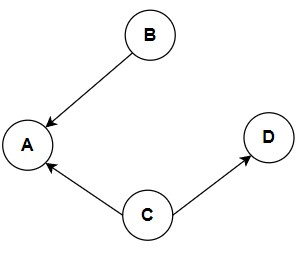
\includegraphics{graph_or.jpg}
        \caption{Ориентированный граф}
    \end{minipage}
    \hspace{3cm}
    \begin{minipage}[t]{4cm}
        \centering
        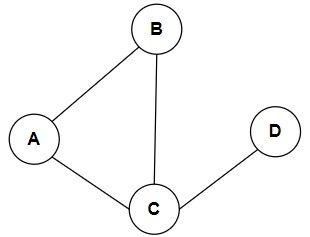
\includegraphics{graph_nor.jpg}
        \caption{Неориентированный граф}
    \end{minipage}
\end{figure*}

\textbf{Степенью} называется количество ребер, соединенных с этой вершиной.
Если степень вершины равна 0, то такая вершина называется \textbf{изолированной}.
Степень вершины может быть \textbf{входящая} и \textbf{исходящая}. Входящая степень вершины $v$
это количество ребер вида $\langle i, v \rangle$, то есть количество ребер которые входят в $v$.
Исходящая степень вершины $v$ это количество ребер вида $\langle v, i \rangle$, то есть количество ребер
которые входят из $v$.

\begin{thm}
    В любом графе всегда найдутся хотя бы две вершины с одинаковой степенью.
\end{thm}

Дуга, у которой начало и конец совпадают, называется \textbf{петлей}.

\textbf{Частичным графом} графа  $\langle M, N \rangle$ называется пара множеств $\langle M, N'\rangle$, где $N'$ - 
подмножество $N$. Пусть $M'$ - какое-либо подмножество $M$. Обозначим через $N(M')$ множество всех
дуг, у которых и начала и концы принадлежат $M'$. Граф $\langle M', N(M')\rangle$ называется \textbf{подграфом} графа $\langle M, N\rangle$.
Граф $\langle M', N'\rangle$ где $N' \subset N(M')$ называется  \textbf{частичным подграфом} графа $\langle M, N\rangle$

\hspace{3mm}

Частичный подграф $\langle M', N'\rangle$ называется \textbf{простым путем}, если
\begin{enumerate}
    \item число его дуг $k$ на единицу меньше числа вершин
    \item можно так пронумеровать $M'$ числами от 0 до $k$ и $N'$ числами от 1 до $k$,
    что для любой дуги $u \in N'$
\end{enumerate}

Пусть $num$ - это номер дуги $u$, а $beg u$ и $end u$ начало и конец дуги соответственно. Тогда:
\begin{equation}
    num(u) = num(end u ) = num(beg u) + 1
\end{equation}
% \begin{figure}
%     \centering 
%     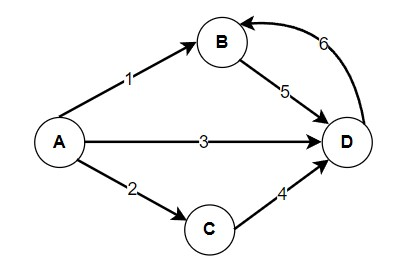
\includegraphics{graph_1.jpg}
%     \caption{Пример графа}
% \end{figure}
